\documentclass[11pt]{article}

% ====================================================
% PACKAGES
% ====================================================
\usepackage[margin=1in, headheight=13.6pt]{geometry}
\usepackage[T1]{fontenc}
\usepackage{lmodern}
\usepackage{microtype}
\usepackage{setspace}
\usepackage{tcolorbox}
\usepackage{amsmath, amssymb, mathtools}
\usepackage{siunitx}
\usepackage{bm}

\usepackage{graphicx}
\usepackage{float}
\usepackage{subcaption}

\usepackage{enumitem}
\usepackage{booktabs}
\usepackage{longtable}
\usepackage{array}
\usepackage{multirow}

\usepackage{xcolor}
\usepackage{hyperref}

\usepackage{fancyhdr}
\usepackage{lastpage}

\usepackage{indentfirst}
\usepackage[justification=centering]{caption}
\usepackage{pdfpages}
\usepackage{listings}

\lstdefinestyle{pystyle}{
    language=Python,
    basicstyle=\ttfamily\small,
    keywordstyle=\color{blue!60!black}\bfseries,
    commentstyle=\color{green!40!black}\itshape,
    stringstyle=\color{orange!70!black},
    numbers=left,
    numberstyle=\tiny\color{gray},
    numbersep=6pt,
    breaklines=true,
    breakatwhitespace=false,
    showstringspaces=false,
    frame=single,
    rulecolor=\color{gray!50},
    tabsize=4
}
\lstset{style=pystyle}

\pagestyle{fancy}
\fancyhf{}
\lhead{\Assignment\ |\ \course}
\rhead{\Name\ |\ \today}
\cfoot{Page \thepage\ of~\pageref{LastPage}}

\hypersetup{
    colorlinks,
    linkcolor={red!50!black},
    citecolor={blue!50!black},
    urlcolor={blue!80!black}
}

\newcommand{\Name}{Arael Anaya}
\newcommand{\Assignment}{Homework 2}
\newcommand{\course}{Robot Mechanics}

% Boxed final-answer environment
\newtcolorbox{result}{
    colback=blue!3!white,
    colframe=blue!40!black,
    boxrule=0.6pt,
    arc=2pt,
    left=6pt, right=6pt, top=4pt, bottom=4pt
}

% Boxed problem-statement environment
\newtcolorbox{statement}{
    colback=gray!5!white,
    colframe=gray!50!black,
    boxrule=0.4pt,
    arc=2pt,
    left=6pt, right=6pt, top=4pt, bottom=4pt
}

% Visible placeholder for work not yet added
\newcommand{\workplaceholder}{%
    \par\vspace{4pt}\noindent\textcolor{gray!60}{\itshape [Work not yet added: paste solution here]}\par\vspace{4pt}%
}

% Boxed correction-note environment (flags a fix made to the original hand calc)
\newtcolorbox{fixnote}{
    colback=orange!5!white,
    colframe=orange!55!black,
    boxrule=0.5pt,
    arc=2pt,
    left=6pt, right=6pt, top=4pt, bottom=4pt,
    fontupper=\small
}

% Notation macros (matching course conventions)
\newcommand{\T}{\bm{T}}
\newcommand{\R}{\bm{R}}
\newcommand{\dvec}{\bm{d}}
\newcommand{\framen}[1]{\{#1\}}
\newcommand{\khat}{\widehat{\bm{k}}}
\newcommand{\wvec}{\bm{\omega}}
\newcommand{\Rotx}{\operatorname{Rot}_x}
\newcommand{\Roty}{\operatorname{Rot}_y}
\newcommand{\Rotz}{\operatorname{Rot}_z}
\newcommand{\atantwo}{\operatorname{atan2}}
\newcommand{\skewx}[1]{\left[#1\right]_{\times}}

\begin{document}

% ====================================================
% PROBLEM 1
% ====================================================
\section*{Problem 1}

\begin{statement}
Given the Euler angle set $\{$Roll $(\psi)$, Pitch $(\theta)$, Yaw $(\phi)\}$: $\Rotz(\phi)\Roty(\theta)\Rotx(\psi)$:
\begin{enumerate}[label=(\alph*), leftmargin=1.6em, itemsep=2pt]
    \item Derive the resulting rotation matrix in terms of $\phi$, $\theta$, and $\psi$.
    \item Provide the inverse solution. In other words, given a rotation matrix $\R = [r_{ij}]$, determine the formulas for $\phi$, $\theta$, and $\psi$ in terms of the entries in $\R$.
    \item At what value of which angle $\phi$, $\theta$, $\psi$ does the inverse solution degenerate? What happens to the remaining two angles?
    \item Using a sketch of the intermediate rotations to assist, describe why this is a degeneracy.
\end{enumerate}
\end{statement}

\subsection*{Part (a): Forward Rotation Matrix}
The three elementary rotations are
\[
    \Rotz(\phi) = \begin{bmatrix}c\phi & -s\phi & 0\\ s\phi & c\phi & 0\\ 0 & 0 & 1\end{bmatrix},\qquad
    \Roty(\theta) = \begin{bmatrix}c\theta & 0 & s\theta\\ 0 & 1 & 0\\ -s\theta & 0 & c\theta\end{bmatrix},\qquad
    \Rotx(\psi) = \begin{bmatrix}1 & 0 & 0\\ 0 & c\psi & -s\psi\\ 0 & s\psi & c\psi\end{bmatrix}.
\]
Multiplying the right-hand pair first,
\[
    \Roty(\theta)\Rotx(\psi) = \begin{bmatrix}
        c\theta & s\theta s\psi & s\theta c\psi\\
        0 & c\psi & -s\psi\\
        -s\theta & c\theta s\psi & c\theta c\psi
    \end{bmatrix},
\]
and then pre-multiplying by $\Rotz(\phi)$:
\begin{result}
\[
    \R(\psi,\theta,\phi) = \begin{bmatrix}
        c\phi c\theta & c\phi s\theta s\psi - s\phi c\psi & c\phi s\theta c\psi + s\phi s\psi\\
        s\phi c\theta & s\phi s\theta s\psi + c\phi c\psi & s\phi s\theta c\psi - c\phi s\psi\\
        -s\theta & c\theta s\psi & c\theta c\psi
    \end{bmatrix}
\]
\end{result}

\subsection*{Part (b): Inverse Solution}
From the third row and first column of the result above,
\[
    s\theta = -r_{31}, \qquad
    c\theta = \pm\sqrt{r_{11}^{2}+r_{21}^{2}}
    \quad\text{since}\quad
    r_{11}^{2}+r_{21}^{2} = c\phi^{2}c\theta^{2}+s\phi^{2}c\theta^{2} = c\theta^{2}.
\]
With $c\theta$ known, the first column gives $\phi$ and the third row gives $\psi$:
\begin{result}
\[
    \theta = \atantwo\!\left(-r_{31},\ \pm\sqrt{r_{11}^{2}+r_{21}^{2}}\right)
\]
\[
    \phi = \atantwo\!\left(\frac{r_{21}}{c\theta_{\pm}},\ \frac{r_{11}}{c\theta_{\pm}}\right),
    \qquad
    \psi = \atantwo\!\left(\frac{r_{32}}{c\theta_{\pm}},\ \frac{r_{33}}{c\theta_{\pm}}\right)
\]
\end{result}
The $\pm$ on the square root gives the two standard solution branches.

\subsection*{Part (c): Degeneracy}
\begin{result}
The solution degenerates at $\theta = \dfrac{\pi}{2} + \pi n$ (a \SI{90}{\degree} pitch).
\end{result}
At that pitch $c\theta = 0$, so $r_{11}=r_{21}=r_{32}=r_{33}=0$ and both the $\phi$ and $\psi$ expressions become $\atantwo(0/0,\,0/0)$. It becomes impossible to find their individual values, only their sum or difference.

\subsection*{Part (d): Why It Is a Degeneracy}
\begin{figure}[H]
    \centering
    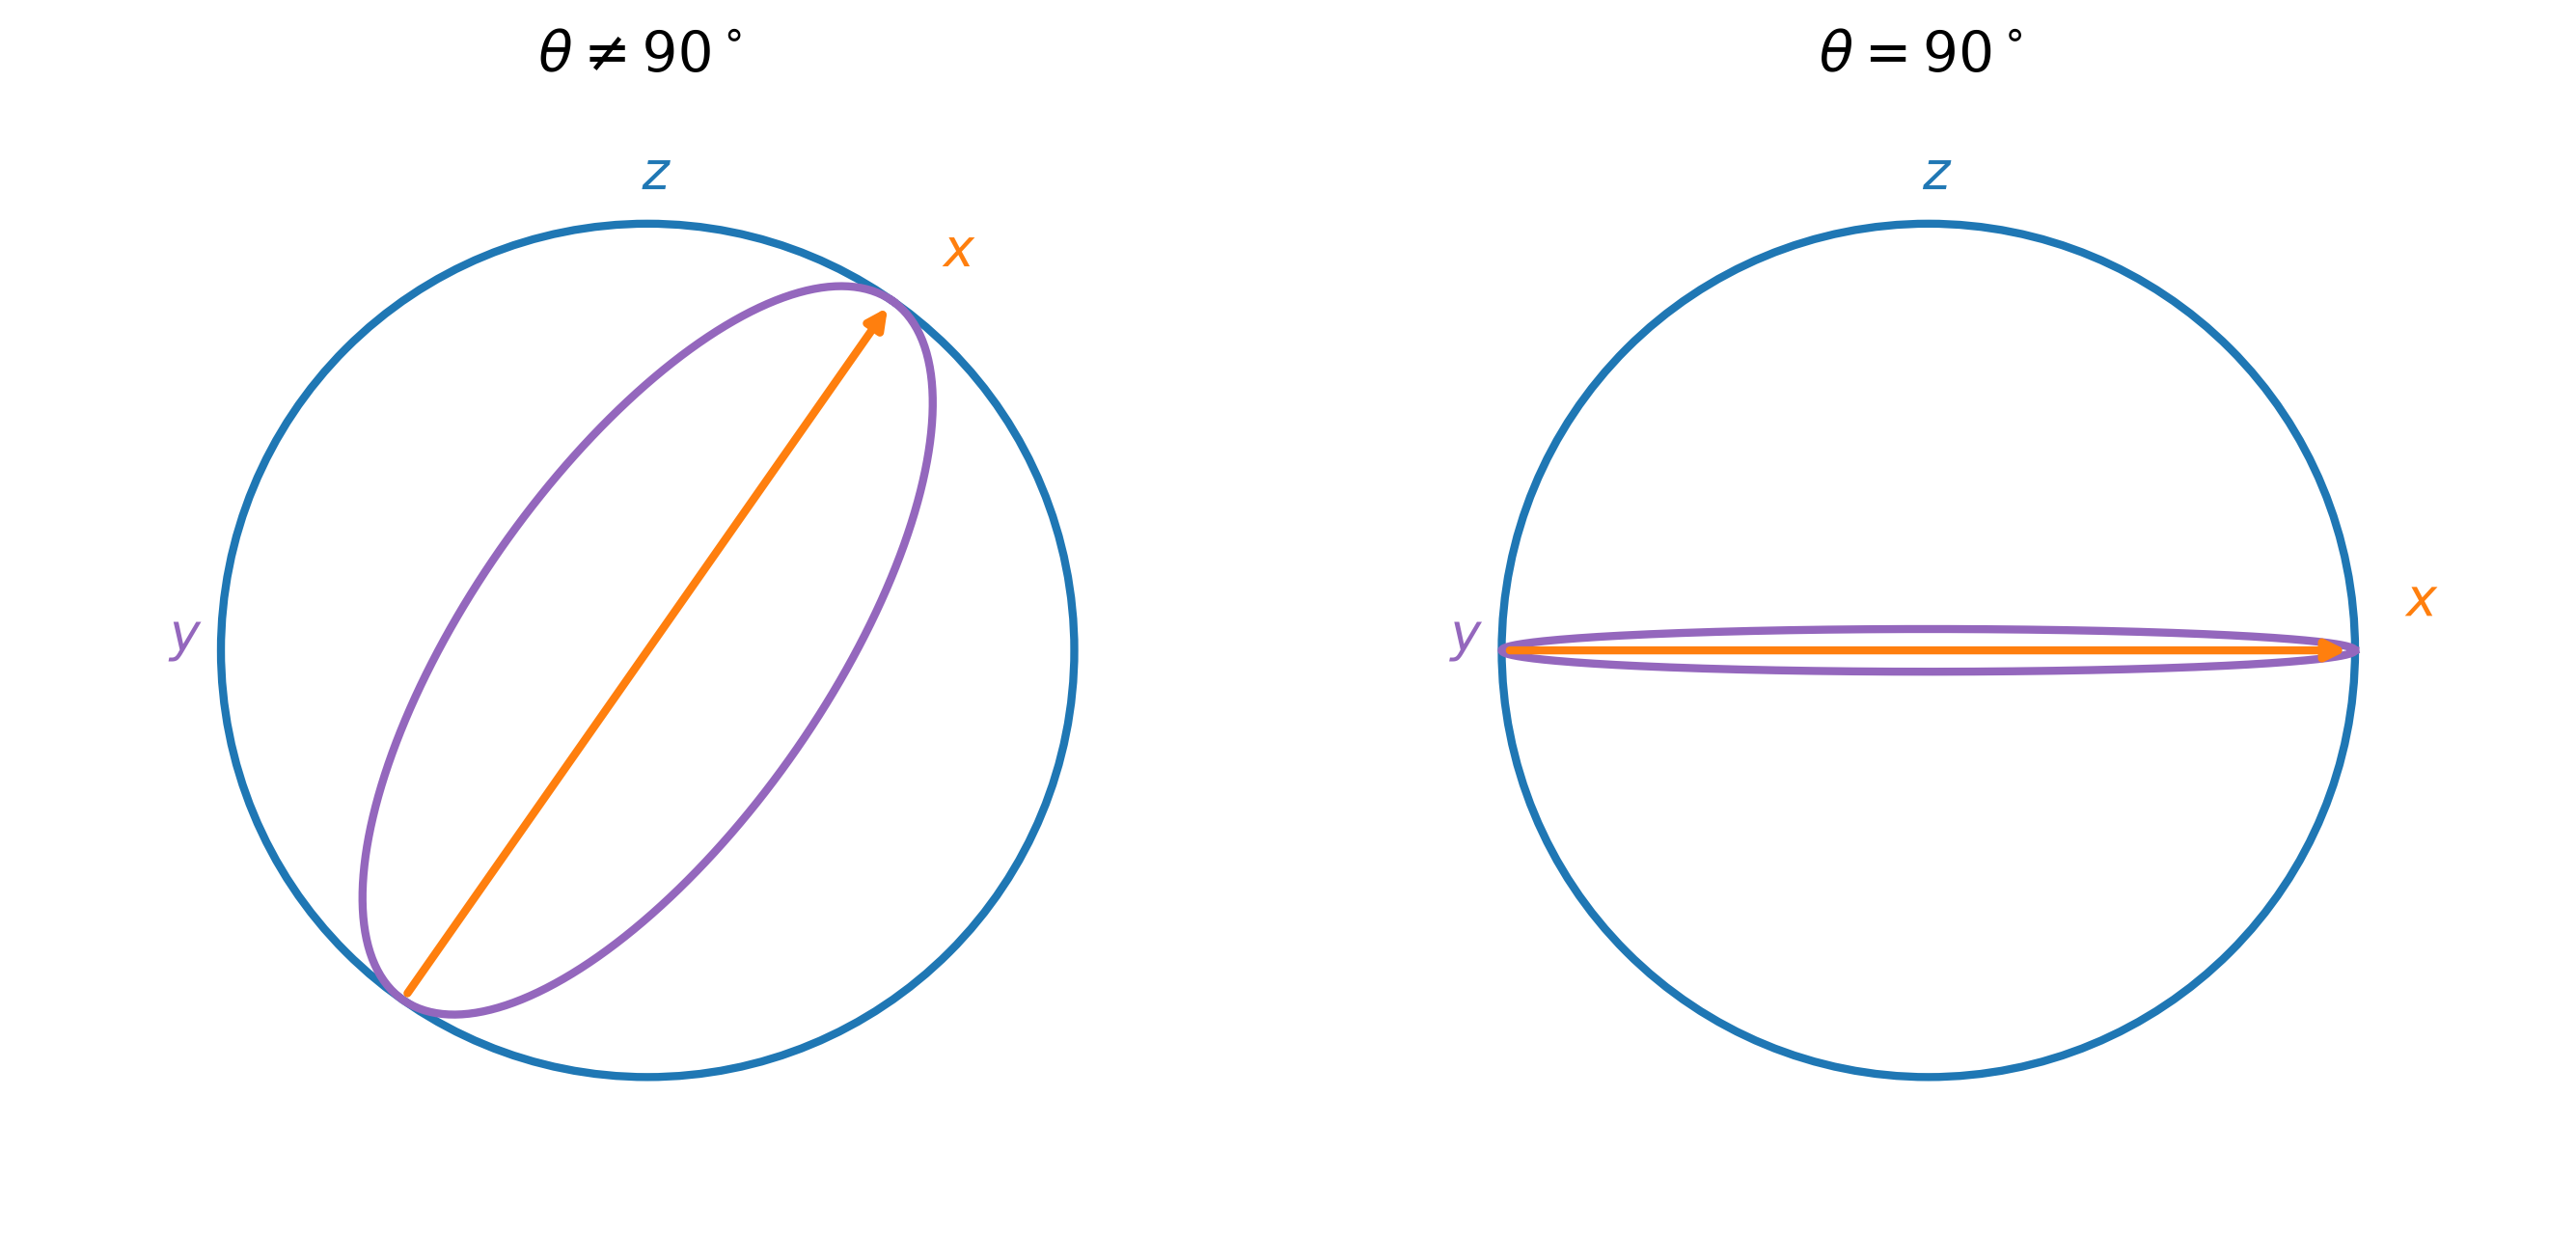
\includegraphics[width=0.8\linewidth]{Figures/Problem1D.png}
    \caption{Intermediate rotations. At left ($\theta\neq\SI{90}{\degree}$) the roll axis $\hat{\bm x}$ and the yaw axis $\hat{\bm z}$ are independent. At right ($\theta=\SI{90}{\degree}$) the roll axis has been pitched into alignment with the yaw axis.}
\end{figure}
When you rotate pitch to \SI{90}{\degree}, the roll axis becomes parallel with the yaw axis, so any rotation from then on spins both. The two rotations are no longer independent: only the combined angle acts on the body, which is why the inverse solution can recover the sum/difference but not $\phi$ and $\psi$ separately. Substituting $\theta = \pi/2$ into part (a) gives,
\[
    \R\left(\psi,\tfrac{\pi}{2},\phi\right) = \begin{bmatrix}
        0 & s(\psi-\phi) & c(\psi-\phi)\\
        0 & c(\psi-\phi) & -s(\psi-\phi)\\
        -1 & 0 & 0
    \end{bmatrix},
\]
which depends on $\phi$ and $\psi$ only through the difference $\psi-\phi$.

% ====================================================
% PROBLEM 2
% ====================================================
\newpage
\section*{Problem 2}

\begin{statement}
Given the following rotation matrix,
\[
    \R = \begin{bmatrix}
        0.6533 & 0.6403 & 0.4040\\
        -0.3488 & 0.7282 & -0.5900\\
        -0.6719 & 0.2445 & 0.6991
    \end{bmatrix},
\]
\begin{enumerate}[label=(\alph*), leftmargin=1.6em, itemsep=2pt]
    \item Prove that it is a rotation matrix.
    \item What are the ZYZ angles for this rotation matrix?
    \item What is the angle and axis representation for this rotation matrix?
    \item What is the Quaternion representation?
\end{enumerate}
\end{statement}

\subsection*{Part (a): Proof That $\R$ Is a Rotation}
A matrix is a rotation if it is orthonormal with a determinant of $+1$. Evaluating both conditions:
\begin{result}
\[
    \det(\R) = 1, \qquad \R\,\R^{T} \approx \bm I
\]
\end{result}
(Evaluated by calculator; the residual in $\R\R^{T}-\bm I$ is only round-off from the four-digit entries.) Since the columns are mutually orthogonal unit vectors and the determinant is $+1$ rather than $-1$, $\R$ is a proper rotation.

\subsection*{Part (b): ZYZ Euler Angles}
For $\R = \Rotz(\phi)\Roty(\theta)\Rotz(\psi)$:
\[
    \theta_{\pm} = \atantwo\!\left(\pm\sqrt{r_{13}^{2}+r_{23}^{2}},\ r_{33}\right), \qquad
    \phi = \atantwo\!\left(\frac{r_{23}}{s\theta_{\pm}},\ \frac{r_{13}}{s\theta_{\pm}}\right), \qquad
    \psi = \atantwo\!\left(\frac{r_{32}}{s\theta_{\pm}},\ \frac{-r_{31}}{s\theta_{\pm}}\right)
\]
Taking the positive branch:
\begin{result}
\[
    \theta = 45.65^\circ, \qquad \phi = -55.60^\circ, \qquad \psi = 20.00^\circ
\]
\end{result}

\subsection*{Part (c): Angle--Axis Representation}
\[
    \theta = \atantwo\!\left(\frac{1}{2}\left\lVert\begin{bmatrix}r_{32}-r_{23}\\ r_{13}-r_{31}\\ r_{21}-r_{12}\end{bmatrix}\right\rVert_{2},\ \frac{\operatorname{tr}(\R)-1}{2}\right), \qquad
    \khat = \frac{1}{2s\theta}\begin{bmatrix}r_{32}-r_{23}\\ r_{13}-r_{31}\\ r_{21}-r_{12}\end{bmatrix}
\]
\begin{result}
\[
    \theta = 57.30^\circ, \qquad \khat = \begin{bmatrix}0.496\\ 0.639\\ -0.588\end{bmatrix}
\]
\end{result}

\subsection*{Part (d): Quaternion Representation}
\[
    q_{0} = \pm\sqrt{\frac{1+\operatorname{tr}(\R)}{4}}, \qquad
    q_{1} = \frac{r_{32}-r_{23}}{4q_{0}}, \qquad
    q_{2} = \frac{r_{13}-r_{31}}{4q_{0}}, \qquad
    q_{3} = \frac{r_{21}-r_{12}}{4q_{0}}
\]
\begin{result}
\[
    Q = \left[\,0.878,\ \begin{bmatrix}0.238 & 0.307 & -0.282\end{bmatrix}^{T}\right]
\]
\end{result}

% ====================================================
% PROBLEM 3
% ====================================================
\section*{Problem 3}

\begin{statement}
What is the rotation matrix and angle-axis vector ($\bm\Omega = \khat\theta$) that are described by the following quaternions:
\begin{enumerate}[label=(\alph*), leftmargin=1.6em, itemsep=2pt]
    \item $[1,[0\quad 0\quad 0]^{T}]$
    \item $[0,[0\quad 0\quad 1]^{T}]$
    \item $[0,[1\quad 0\quad 0]^{T}]$
    \item $[0.5332,[0.5928\quad 0.08311\quad 0.5978]^{T}]$
\end{enumerate}
\end{statement}

Each quaternion $[q_{0},[q_{1}\ q_{2}\ q_{3}]^{T}]$ maps to a rotation by
\[
    \R = \begin{bmatrix}
        1-2(q_{2}^{2}+q_{3}^{2}) & 2(q_{1}q_{2}-q_{0}q_{3}) & 2(q_{1}q_{3}+q_{0}q_{2})\\
        2(q_{1}q_{2}+q_{0}q_{3}) & 1-2(q_{1}^{2}+q_{3}^{2}) & 2(q_{2}q_{3}-q_{0}q_{1})\\
        2(q_{1}q_{3}-q_{0}q_{2}) & 2(q_{2}q_{3}+q_{0}q_{1}) & 1-2(q_{1}^{2}+q_{2}^{2})
    \end{bmatrix},
\]
\[
    \theta = 2\arccos(q_{0}), \qquad
    \khat = \frac{1}{\sin(\theta/2)}\begin{bmatrix}q_{1}\\ q_{2}\\ q_{3}\end{bmatrix}.
\]

\subsection*{Part (a): $[1,[0\ 0\ 0]^{T}]$}
\begin{result}
\[
    \R = \begin{bmatrix}1 & 0 & 0\\ 0 & 1 & 0\\ 0 & 0 & 1\end{bmatrix}, \qquad
    \theta = 0^\circ, \qquad \khat = \vec 0
\]
\end{result}
This is the identity quaternion: there is no rotation, so the axis is arbitrary (taken as $\vec 0$) and $\bm\Omega = \khat\theta = \vec 0$.

\subsection*{Part (b): $[0,[0\ 0\ 1]^{T}]$}
\begin{result}
\[
    \R = \begin{bmatrix}-1 & 0 & 0\\ 0 & -1 & 0\\ 0 & 0 & 1\end{bmatrix}, \qquad
    \theta = 180^\circ, \qquad \khat = \begin{bmatrix}0\\ 0\\ 1\end{bmatrix}
\]
\end{result}

\subsection*{Part (c): $[0,[1\ 0\ 0]^{T}]$}
\begin{result}
\[
    \R = \begin{bmatrix}1 & 0 & 0\\ 0 & -1 & 0\\ 0 & 0 & -1\end{bmatrix}, \qquad
    \theta = 180^\circ, \qquad \khat = \begin{bmatrix}1\\ 0\\ 0\end{bmatrix}
\]
\end{result}

\subsection*{Part (d): $[0.5332,[0.5928\ 0.08311\ 0.5978]^{T}]$}
\begin{result}
\[
    \R = \begin{bmatrix}
        0.271 & -0.539 & 0.797\\
        0.736 & -0.418 & -0.533\\
        0.620 & 0.732 & 0.283
    \end{bmatrix}, \qquad
    \theta = 115.56^\circ, \qquad \khat = \begin{bmatrix}0.701\\ 0.098\\ 0.707\end{bmatrix}
\]
\end{result}

% ====================================================
% PROBLEM 4
% ====================================================
\section*{Problem 4}

\begin{statement}
An object is spinning with some constant angular velocity $\prescript{0}{}{\wvec}$ such that after time $t$ it has rotated $\theta = \lVert\wvec\rVert_{2}t$ radians about $\prescript{0}{}{\khat} = \prescript{0}{}{\wvec}/\lVert\wvec\rVert_{2}$. Its orientation is then $\prescript{0}{}{\R}_{obj} = \prescript{0}{}{\R}_{i}(\theta,\khat)\,\prescript{i}{}{\R}_{obj}$. Using the angle-axis representation, derive $\dot{\R} = \mathrm{d}\R/\mathrm{d}t$, which by the chain rule yields
\[
    \frac{\mathrm{d}\R}{\mathrm{d}t} = \left(\frac{\mathrm{d}}{\mathrm{d}\theta}\prescript{0}{}{\R}_{i}(\theta,\khat)\,\prescript{i}{}{\R}_{obj}\right)\dot{\theta}
    + \left(\frac{\mathrm{d}}{\mathrm{d}\khat}\prescript{0}{}{\R}_{i}(\theta,\khat)\,\prescript{i}{}{\R}_{obj}\right)\dot{\khat},
\]
and evaluate at $\theta = t = 0$, before the orientation is modified by rotation.
\end{statement}

\subsection*{Setup: Rodrigues' Formula}
From (3.41) in Hollerbach's notes,
\[
    \R_{\khat}(\theta) = \bm I\,c\theta + \skewx{\khat}s\theta + \khat\khat^{T}(1-c\theta).
\]

\subsection*{The Two Chain-Rule Terms}
\[
    \frac{\mathrm{d}\R}{\mathrm{d}t}
    = \left(\frac{\mathrm{d}}{\mathrm{d}\theta}\prescript{0}{}{\R}_{i}(\theta,\khat)\,\prescript{i}{}{\R}_{obj}\right)\dot\theta
    + \left(\frac{\mathrm{d}}{\mathrm{d}\khat}\prescript{0}{}{\R}_{i}(\theta,\khat)\,\prescript{i}{}{\R}_{obj}\right)\dot{\khat}
\]
The angular velocity is constant, so
\[
    \khat = \frac{\prescript{0}{}{\wvec}}{\lVert\wvec\rVert_{2}},\qquad \frac{\mathrm{d}\wvec}{\mathrm{d}t}=0
    \quad\therefore\quad \dot{\khat} = 0,
\]
which gets rid of the second term. For the first term, $\theta = \lVert\wvec\rVert_{2}t$ gives
\[
    \dot\theta = \frac{\mathrm{d}\theta}{\mathrm{d}t} = \lVert\prescript{0}{}{\wvec}\rVert_{2}.
\]

\subsection*{Differentiating Rodrigues' Formula}
\[
    \frac{\mathrm{d}}{\mathrm{d}\theta}\left(\R_{\khat}(\theta)\right)
    = -\bm I\,s\theta + \skewx{\khat}c\theta + \khat\khat^{T}s\theta
    \qquad\therefore\qquad
    \left.\frac{\mathrm{d}}{\mathrm{d}\theta}\left(\R_{\khat}(\theta)\right)\right|_{\theta=0} = \skewx{\khat}.
\]

\subsection*{Evaluating at $\theta = t = 0$}
Substituting both results,
\[
    \frac{\mathrm{d}\R}{\mathrm{d}t}
    = \left(\underbrace{\frac{\mathrm{d}}{\mathrm{d}\theta}\prescript{0}{}{\R}_{i}(\theta,\khat)}_{\skewx{\khat}}\prescript{i}{}{\R}_{obj}\right)\lVert\prescript{0}{}{\wvec}\rVert_{2}
    = \skewx{\khat}\,\prescript{i}{}{\R}_{obj}\,\lVert\prescript{0}{}{\wvec}\rVert_{2}.
\]
At $\theta = 0$ the incremental rotation is the identity, so the orientation is unmodified:
\[
    \prescript{0}{}{\R}_{obj}(0) = \prescript{0}{}{\R}_{i}(0,\khat)\,\prescript{i}{}{\R}_{obj} = \bm I\cdot\prescript{i}{}{\R}_{obj}
    \qquad\therefore\qquad \prescript{0}{}{\R}_{obj}(0) = \prescript{i}{}{\R}_{obj}.
\]
Finally, the scalar $\lVert\prescript{0}{}{\wvec}\rVert_{2}$ gets multiplied inside the skew operator:
\[
    \lVert\prescript{0}{}{\wvec}\rVert_{2}\skewx{\khat}
    = \lVert\prescript{0}{}{\wvec}\rVert_{2}\left[\frac{\wvec}{\lVert\prescript{0}{}{\wvec}\rVert_{2}}\right]_{\times}
    = \skewx{\wvec}.
\]
\begin{result}
\[
    \frac{\mathrm{d}\R}{\mathrm{d}t} = \skewx{\wvec}\,\prescript{0}{}{\R}_{obj}
\]
\end{result}

% ====================================================
% PROBLEM 5
% ====================================================
\newpage
\section*{Problem 5}

\begin{statement}
Consider the combination of robot, square table, block, and camera below, with associated coordinate systems as shown. The relative locations of robot, table, block, and camera are shown in Fig.~\ref{fig:p5}. The block is located at the center of the table.
\begin{enumerate}[label=(\alph*), leftmargin=1.6em, itemsep=2pt]
    \item Find $\prescript{0}{}{\T}_{1}$, $\prescript{1}{}{\T}_{2}$, $\prescript{2}{}{\T}_{3}$, and $\prescript{0}{}{\T}_{3}$ by inspection.
    \item Assume the block has moved. It is tracked by the camera and is known to exist at location $\prescript{3}{}{\dvec}_{32} = [-0.5\quad 0.5\quad 3]^{T}$. Where is the block in the robot's coordinate system, i.e.\ what is $\prescript{0}{}{\dvec}_{02}$?
\end{enumerate}
\end{statement}

\begin{figure}[H]
    \centering
    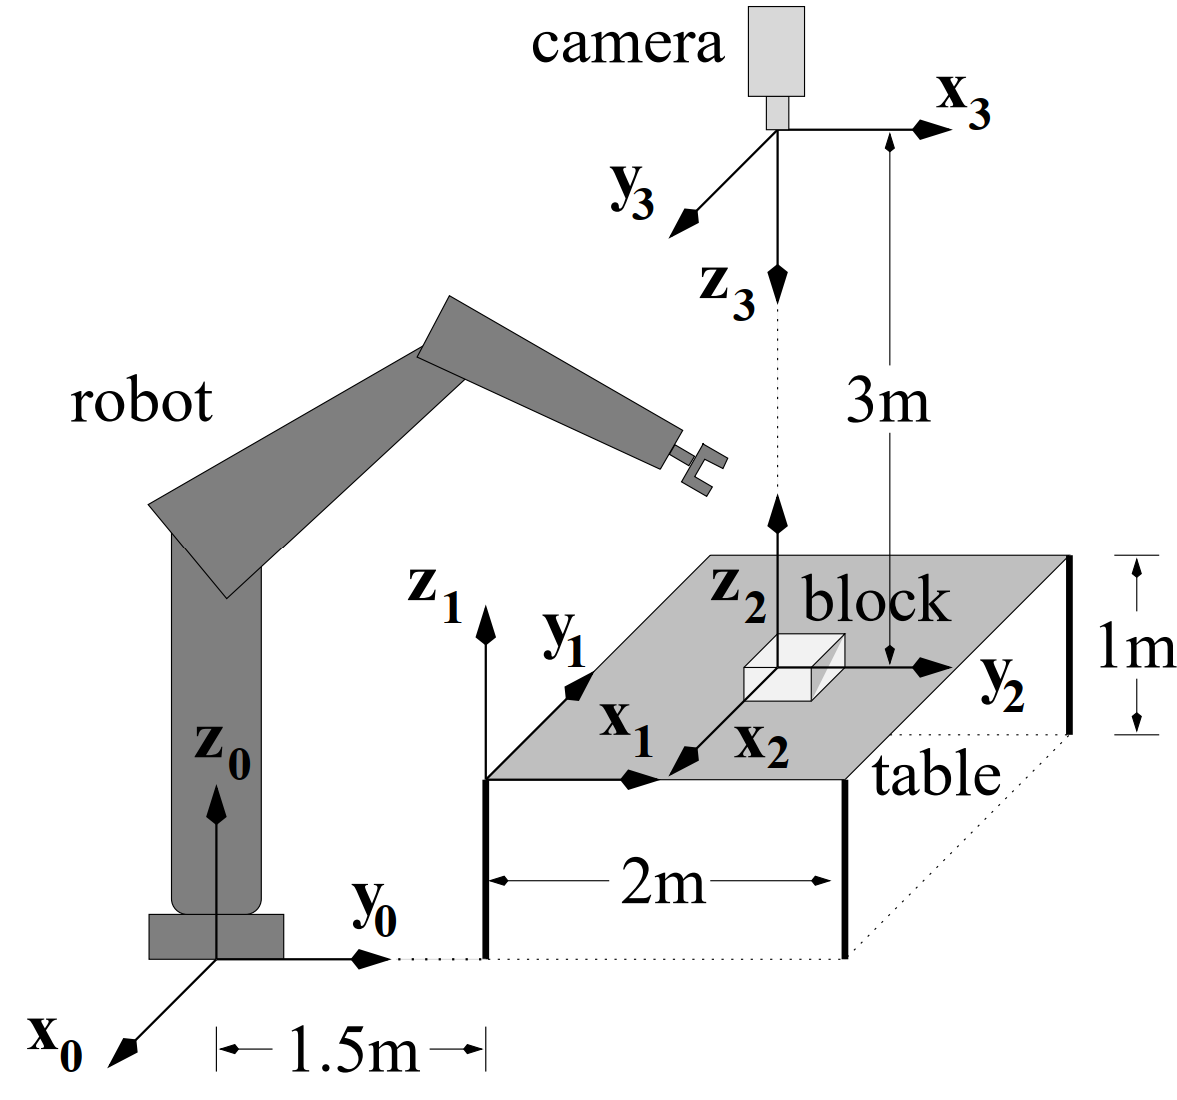
\includegraphics[width=0.45\linewidth]{Figures/robot_arm_table_hollerbach.png}
    \caption{Robot, square table, block, and camera with their associated coordinate systems.}
    \label{fig:p5}
\end{figure}

\subsection*{Part (a): Transforms by Inspection}
\begin{result}
\[
    \prescript{0}{}{\T}_{1} = \begin{bmatrix}
        0 & -1 & 0 & 0\\
        1 & 0 & 0 & 1.5\\
        0 & 0 & 1 & 1\\
        0 & 0 & 0 & 1
    \end{bmatrix},\qquad
    \prescript{1}{}{\T}_{2} = \begin{bmatrix}
        0 & 1 & 0 & 1\\
        -1 & 0 & 0 & 1\\
        0 & 0 & 1 & 0\\
        0 & 0 & 0 & 1
    \end{bmatrix},\qquad
    \prescript{2}{}{\T}_{3} = \begin{bmatrix}
        0 & 1 & 0 & 0\\
        1 & 0 & 0 & 0\\
        0 & 0 & -1 & 3\\
        0 & 0 & 0 & 1
    \end{bmatrix}
\]
\end{result}
Chaining them,
\[
    \prescript{0}{}{\T}_{3} = \prescript{0}{}{\T}_{1}\,\prescript{1}{}{\T}_{2}\,\prescript{2}{}{\T}_{3}
\]
\begin{result}
\[
    \prescript{0}{}{\T}_{3} = \begin{bmatrix}
        0 & 1 & 0 & -1\\
        1 & 0 & 0 & 2.5\\
        0 & 0 & -1 & 4\\
        0 & 0 & 0 & 1
    \end{bmatrix}
\]
\end{result}

\subsection*{Part (b): Block Location in the Robot Frame}
Given $\prescript{3}{}{\dvec}_{32} = [-0.5\quad 0.5\quad 3]^{T}$, map it through $\prescript{0}{}{\T}_{3}$ in homogeneous coordinates:
\[
    \begin{bmatrix}\prescript{0}{}{\dvec}_{02}\\ 1\end{bmatrix}
    = \prescript{0}{}{\T}_{3}\begin{bmatrix}\prescript{3}{}{\dvec}_{32}\\ 1\end{bmatrix}
    = \begin{bmatrix}
        0 & 1 & 0 & -1\\
        1 & 0 & 0 & 2.5\\
        0 & 0 & -1 & 4\\
        0 & 0 & 0 & 1
    \end{bmatrix}
    \begin{bmatrix}-0.5\\ 0.5\\ 3\\ 1\end{bmatrix}
\]
\begin{result}
\[
    \prescript{0}{}{\dvec}_{02} = \begin{bmatrix}-0.5\\ 2\\ 1\end{bmatrix}
\]
\end{result}

% ====================================================
% APPENDIX A: PYTHON CODE
% ====================================================
\newpage
\section*{Appendix A: Python Code}

\subsection*{Problem 1: Gimbal Degeneracy Sketch}
\lstinputlisting[caption={Problem 1.py: generates the intermediate-rotation sketch in Fig.~1.}]{"../Code/Problem 1.py"}

\newpage
\subsection*{Problem 2: ZYZ Angles, Angle--Axis, and Quaternion}
\lstinputlisting[caption={Problem 2.py: evaluates the ZYZ angles, angle-axis pair, and quaternion for Problem 2.}]{"../Code/Problem 2.py"}

\newpage
\subsection*{Problem 3: Quaternion to Rotation Matrix and Angle--Axis}
\lstinputlisting[caption={Problem 3.py: converts each quaternion in Problem 3 to a rotation matrix and angle-axis pair.}]{"../Code/Problem 3.py"}

% ====================================================
% APPENDIX B: HAND CALCULATIONS
% ====================================================
\newpage
\section*{Appendix B: Hand Calculations}

\begin{fixnote}
\textbf{Corrections made when typing up the hand calcs below:}
\begin{enumerate}[leftmargin=1.2em, itemsep=4pt]
    \item \textbf{Problem 1(b), page 1:} the boxed yaw formula was written as $\phi = \atantwo\!\left(\frac{r_{21}}{c\theta_{\pm}},\ \frac{r_{12}}{c\theta_{\pm}}\right)$, but $r_{12}$ doesn't show up in the $\phi$ equation. The correct value comes from the first column, $r_{21} = s\phi c\theta$ and $r_{11} = c\phi c\theta$ (the same terms $c\theta = \sqrt{r_{11}^{2}+r_{21}^{2}}$ above it is built from). 
    \item \textbf{Problem 3(d), page 6:} the $(1,2)$ entry of the rotation matrix was written as $-0.639$. Evaluating $2(q_{1}q_{2}-q_{0}q_{3}) = 2\big((0.5928)(0.08311)-(0.5332)(0.5978)\big)$ gives $-0.539$, matching the neighbouring entries ($0.271$, $0.797$, $0.736$, $-0.418$, $-0.533$, $0.620$, $0.732$, $0.283$) and the boxed axis $\khat = [0.701\ 0.098\ 0.707]^{T}$ exactly.
\end{enumerate}
\end{fixnote}

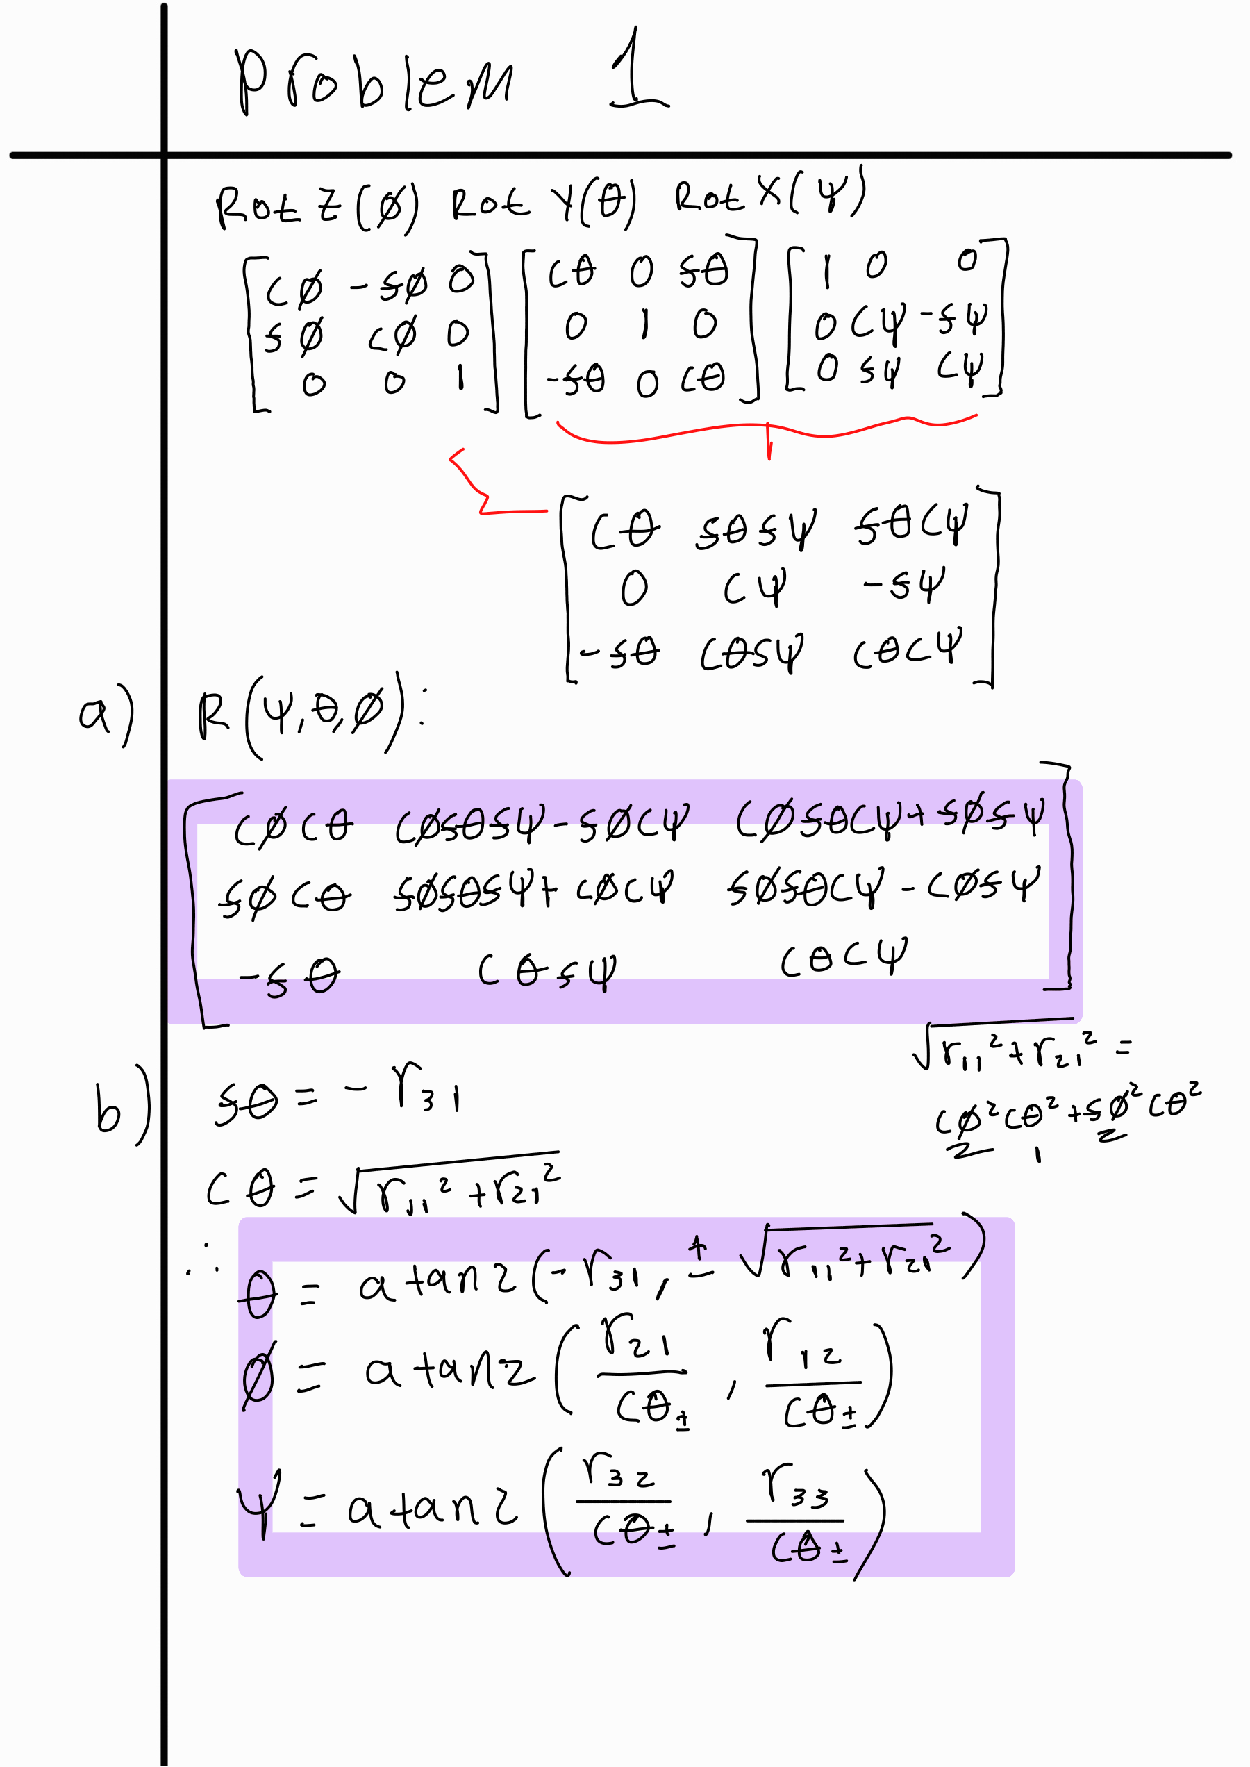
\includepdf[pages=-, pagecommand={\thispagestyle{plain}}, scale=0.9]{../Homework_2_hand_calcs.pdf}

\end{document}
